% !TeX spellcheck = en_GB

\begin{frame}{Election Monitoring with on Twitter~\footfullcite{attarwala_how_2017}}
	\vspace*{-1.2mm}
	\begin{figure}
		\centering
		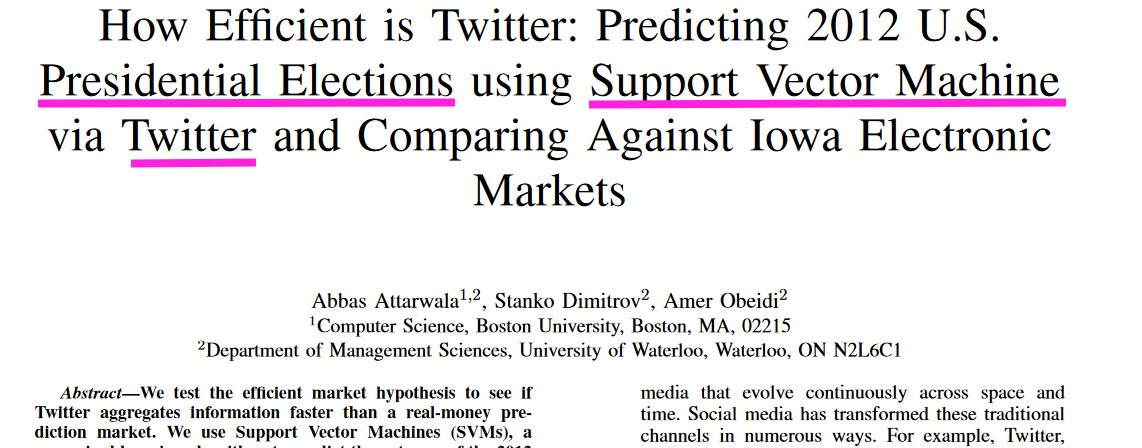
\includegraphics[width=0.9\linewidth, keepaspectratio]{pictures/TwitterElection2012/Twitter_Election_2012_small.png}
	\end{figure}

\end{frame}


\begin{frame}{Prediction}
	\begin{columns}
		
		\begin{column}{0.55\textwidth}
			\begin{tcolorbox}[enhanced jigsaw, colback=white, opacityback=.4, colframe=ElixirPurple, arc=3mm, boxrule=0mm, height=0.8\textheight, valign=center, title=Frequency]
				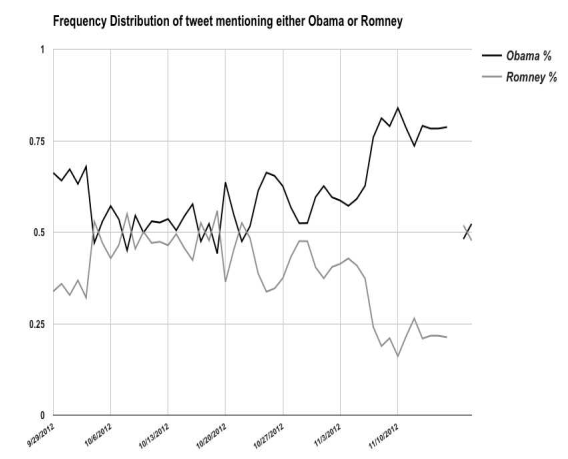
\includegraphics[width=\tcbtextwidth,   keepaspectratio]{pictures/TwitterElection2012/twitter_temp_distr.png}
			\end{tcolorbox}
		\end{column}
		
		\begin{column}{0.55\textwidth}
			\begin{tcolorbox}[enhanced jigsaw, colback=white, opacityback=.4, colframe=ElixirPurple, arc=3mm, boxrule=0mm, height=0.8\textheight, valign=center, title=Prediction]
				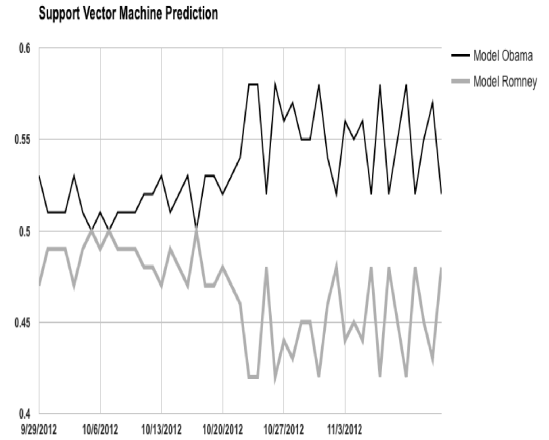
\includegraphics[width=\tcbtextwidth,   keepaspectratio]{pictures/TwitterElection2012/twitter_svm.png}
			\end{tcolorbox}
		\end{column}
		
	\end{columns}
\end{frame}


\begin{frame}{Election on Mastodon}
	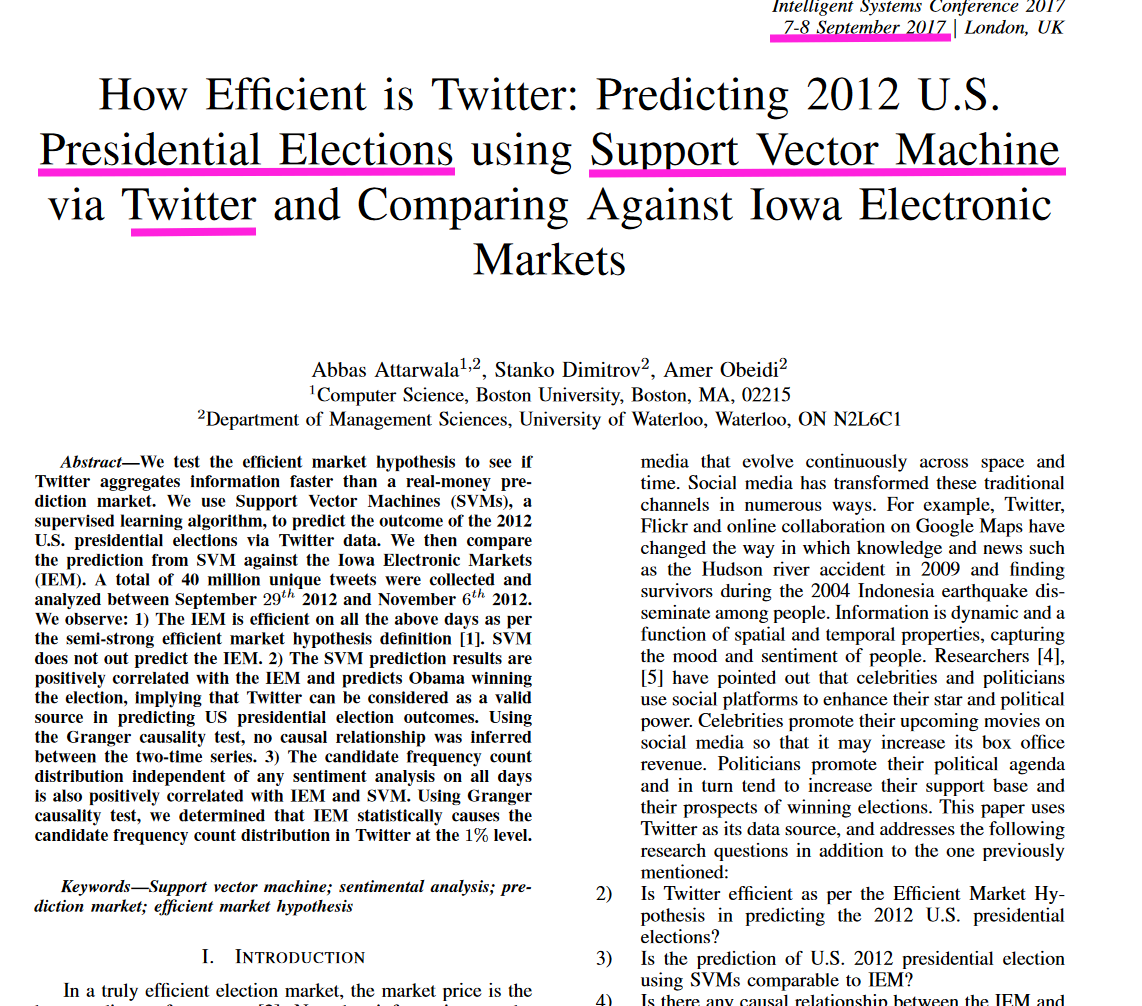
\includegraphics[width=\linewidth, keepaspectratio]{pictures/TwitterElection2012/Twitter_Election_2012.png}
	\postitnote{1.5cm}{-3.5cm}{4.8cm}{Bavarian State Election}
	\postitnote{8.2cm}{-3.5cm}{6.5cm}{Pre-Trained Deep Learning NLP Model}
	
	
	\postitnote{6.1cm}{-2.8cm}{1.8cm}{Mastodon}
	\postitnote{10.8cm}{-2.8cm}{2.5cm}{2023}
	
	\graybar{4.1cm}{-4.1cm}{10.8cm}{2.0cm}
	\postitnote{2.3cm}{-4.2cm}{1.8cm}{Mastodon}
	
\end{frame}
